\section{Enrichment Overview}
% Paper 2
In this context the term \emph{enrichment} describes the extension of the
(semantic) schema of a knowledge base. The process of knowledge base enrichment increases the
semantic richness and the expressiveness of an ontology. 
The goal of the enrichment progress is to find  additional axioms, which can be
added to an existing ontology. A special case is to find definition of classes and
subclasses. This process is closely related to the Inductive Logic Programming
(ILP) as described later in this article.
Ontology enrichment methods usually depend on machine learning or on applying
heuristics to find additional axioms for the knowledge graph. \cite{paper2}

As stated before, knowledge base enrichment usually works on existing data to
improve the semantic schema. It supports the so called \emph{grass-root}
approach for creating ontologies. Here the whole ontology structure is not
created upfront, but evolves over time and with every part of data that is added to the
knowledge base.\cite{paper2}

\begin{figure*}
\centering
\label{venn}
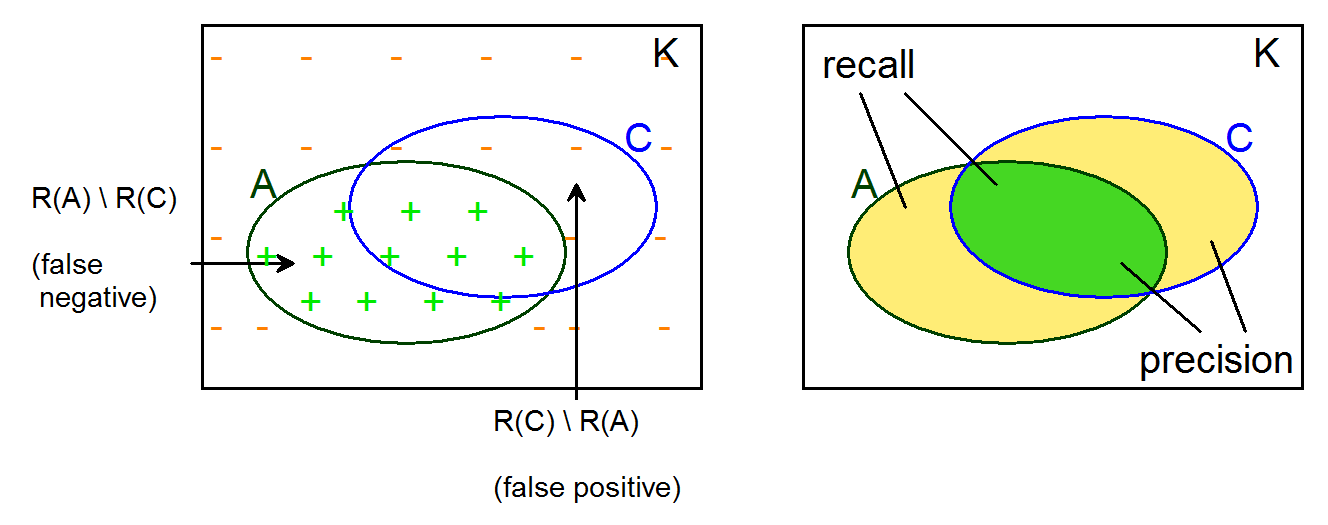
\epsfig{file=img/venn.png, width = 14 cm}
\caption{This figure visualises the class $A$ and the expression to test $C$ as
a Venn diagram. It also shows the the terms \emph{recall} and \emph{precision}.
(Based on the figure in \cite{paper1})}
\end{figure*}



%=====================================================================================
%=====================================================================================
%=====================================================================================
\newpage
\section{Class Learning}
% Paper 1
\subsection{Motivation}
The class learning approach is one method of enrichment in knowledge bases. It
aims at finding new definition of classes to extend the semantic schema. For the
motivation of this method examine the following example.

\begin{example}
For this example consider a knowledge base containing a class \texttt{President
of the United States} with instance data like Abraham Lincoln, John F. Kennedy,
Bill Clinton and Barack Obama. A class Learning algorithm may suggest that the
President class is equivalent to the following two class expressions: \footnote{The
class 'American citizen' is here a subclass of 'Person', which makes the second
statement more specific.}
\vspace{-0.60 cm}
\begin{verbatim}
	1) Person and born in the USA
	2) American citizen and born in the USA
\end{verbatim}
\vspace{-0.40 cm}
\end{example}

These suggestions would then be presented to a knowledge engineer who than can
decide if they are plausible and therefore should be added to the knowledge
graph or should be discarded.
Should the engineer for instance choose the second statement, he could check if
there are instances of the class \texttt{President}, where the individual is not
also of type American citizen. This could indicate an error or missing
information in the knowledge graph. This could then be fixed in this
semi-automated approach by the knowledge engineer.


\subsection{Learning Problem}
The problem of learning class definitions for given data depend on the so called
inductive reasoning as opposed to inference or deductive reasoning.\cite{paper1}
Inductive Reasoning is also a key concept in Inductive Logic Programming (ILP).


\begin{definition}
We are searching for a formal description of the class $A$, which has existing
instances in the examined ontology. A possible class expression $C$ then
contains axioms of the form $A \subseteq C$ or $A \equiv C$.
\end{definition}

This means that the learned expression $C$ is a description of the individuals
of $A$. In our president example, the individuals are the presidents John F.
Kennedy, Barack Obama etc. whereas $C$ can be one of the suggested expression.
In many cases there will be no exact solution for $C$, but rather an
approximation. This can be the case, if the knowledge base contains false class
assignments or missing information. In our example the birthplace of Thomas
Jefferson might be missing in the ontology. However, if most of the other
presidents have the correct birthplace the learning algorithm may still suggest
the expressions. Again, missing information may then be completed by the
knowledge engineer.

In a complex knowledge base the class learning algorithm may find many new class
definition and often very complicated expression for the same class. Based on
Occam's razor \cite{occam-razor} simple solutions are preferred over complex ones,
because they are more readable an thus easier for the knowledge engineer to
evaluate. Simplicity is measured in an straight forward way: the length of an
expression, which consists of role, concept and quantifiers.
The algorithm presented in \cite{paper1} is strongly biased towards shorter
expressions.

\subsection{Algorithm}
One algorithm for solving the learning problem is called CELOE (Class
Expression Learning for Ontology Engineering). It is described in \cite{paper1}.
A brief overview of CELOE is given in Figure 2.
\begin{figure}
\label{celoe}
\centering
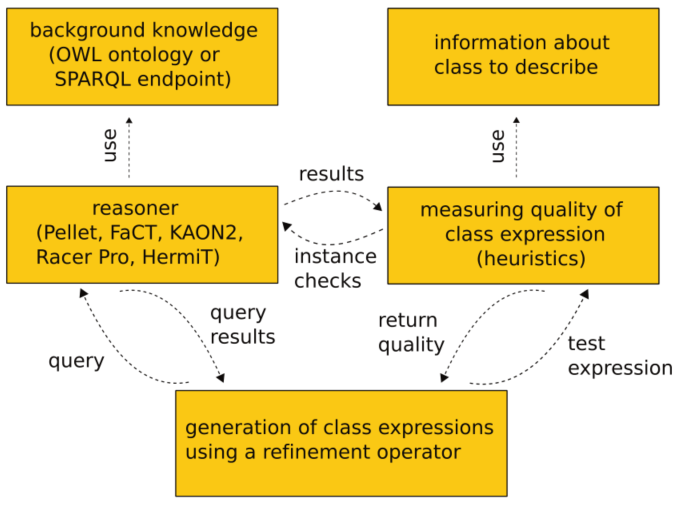
\epsfig{file=img/celoe.png, width = 8 cm}
\caption{Schematic overview of the CELOE algorithm.\cite{paper1}}
\end{figure}
The algorithm follows the ``generate and test'' approach which is the common
concept in ILP.\cite{Foundation_ILP} 
During the learning process many class expression are created and tested against
the background knowledge. Each of these class expressions is evaluated using
different heuristics which are described in detail in chapter 5.

To find appropriate class expression for describing existing classes, CELOE uses
a so called \emph{refinement operator}. The idea of this operator is based on
the work in \cite{refinement1},\cite{refinement2} and \cite{refinement3}. Refinement
operators are used to search in the space of expressions in a knowlege base. It
can be seen as a top-down algorithm and is illustrated in Figure 3.
As an example consider the following path ($\leadsto$ indicates a refinement
step):\vspace{4pt}\\
$T \leadsto Person \leadsto Person \sqcap takesPartIn.T \leadsto Person \sqcap
takesPartIn.Meeting$

\begin{figure}
\label{tree}
\centering
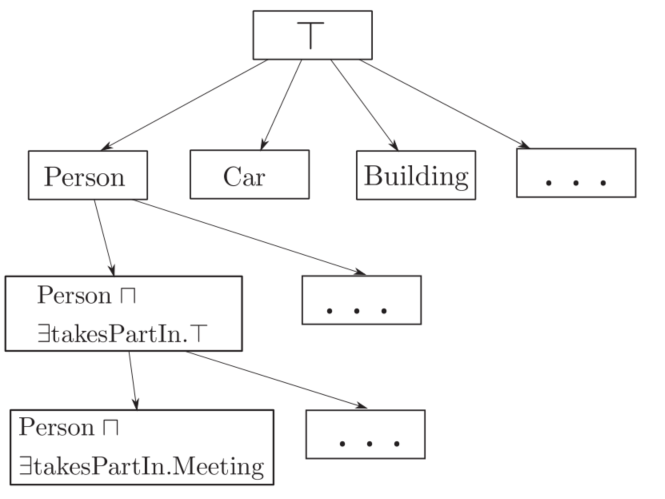
\epsfig{file=img/tree.png, width = 8 cm}
\caption{A search tree for class expressions is the basis of the
refinement operator.\cite{paper1}}
\end{figure}


%=====================================================================================
%=====================================================================================
%=====================================================================================
\newpage
\section{Enrichment with OWL Axioms}
% Paper 2
OWL offers many different types of axioms. The method described in \cite{paper2}
uses many different types to enrich the knowledge base. 
\begin{figure}
\label{3-Phase}
\centering
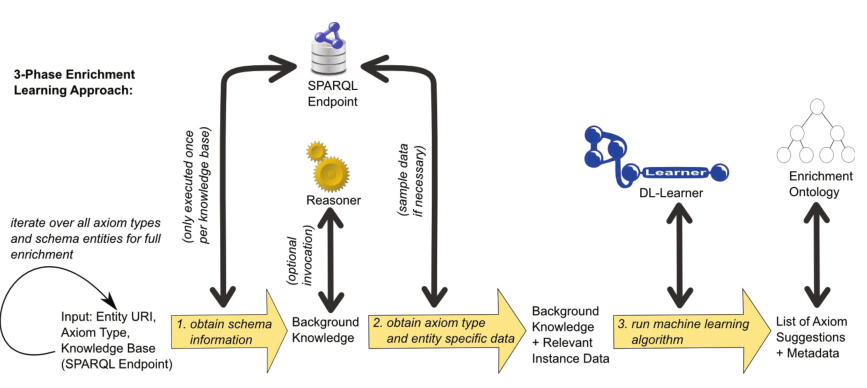
\epsfig{file=img/3-phase-enrichment.png, width = 8 cm}
\caption{3-Phase Enrichment Workflow\cite{paper2}}
\end{figure}
Figure 4 shows the 3 steps in the enrichment workflow:
\begin{enumerate}
  \item The first phase is about obtaining general information in the
  knowledge base. In particular axioms, which define the class hierarchy, are
  obtained. The schema is queried via SPARQL, but have to be loaded only once.
  The result is stored in memory.
  \item In the second phase, data is again obtained via SPARQL. These background
  checks allows the method to learn and test new axioms. Examples for different
  axiom types are explained in the following section.
  \item The score of the axiom candidates is computed and the result can be
  evaluated by a knowledge engineer.
\end{enumerate}

The algorithm for suggestion of new axioms is based on checking and counting RDF
triples. In the following example we want to learn if the class $A$ is an
appropriate domain of a predicate $p$. For that we count the triples that match
this statement to obtain a score. 

\begin{example}
Lets look at the predicate \texttt{onto:attendsMeeting} and check if we can find
a suitable candidate for a domain. Note that \texttt{onto:Manager} is a subclass
of \texttt{onto:Employee}.
\end{example}
\begin{lstlisting}[morekeywords={onto, rdf, rdfs}, caption=Triples written in
turtle syntax] @PREFIX onto: <http://ontology-to-enrich.com/>.
onto:Software_Engineer		
		onto:attendsMeeting 	onto:TeamMeeting;
		rdf:type				onto:Employee.
onto:Software_Architekt		
		onto:attendsMeeting 	onto:TeamMeeting;
		rdf:type				onto:Employee.
onto:Project_Manager		
		onto:attendsMeeting 	onto:ManagerMeeting;
		rdf:type				onto:Manager.
		
onto:Manager   rdfs:subClassOf	onto:Employee.
\end{lstlisting}
Looking at this example we would obtain a score of 33.3 \% (1 out of 3) for the
class \texttt{onto:Manager} and 100 \% (3 out of 3) for the class
\texttt{onto:Employee}.\\
Obviously this extreme simple and straightforward method of calculating the score
has some limitation.
Mainly because the method doesn't discriminate between a score calculated by
having 100 out of 100 correct observations or only 3 out of 3. Different methods, for
example the Wald method \cite{wald-method}, overcome that problem. 
More involved heuristics are also shown in the next chapter. 

\subsection{Obtaining Axioms via SPARQL queries}
This section explains how SPARQL queries are used to extract information in the
second step of the enrichment workflow.

%===============================================================================
%===========================     TABLE     =====================================
% ==============================================================================
\begin{table*}[ht]
\centering
\label{table-heuristic}
\caption{Various examples to illustrate the scores of different heuristics.}
\begin{tabular}{p{3.5 cm} p{3.5 cm} p{2 cm} p{2 cm} p{2 cm} p{2 cm}} \hline
\textbf{Illustration} & \textbf{accuracy \& recall} & \textbf{pred. acc.} &
\textbf{F-Measure} & \textbf{A-Measure} & \textbf{Jaccard}\\
\hline\hline

\raisebox{-.5\height}{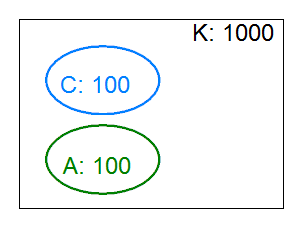
\includegraphics[scale=0.3] {img/table-img1.png}}
& 
\begin{tabular}{l l}accuracy& 0\%\\\\ recall & 0\%\end{tabular}
& 80 \% & 0 \% & 0 \% & 0 \% \\ \hline 

\raisebox{-.5\height}{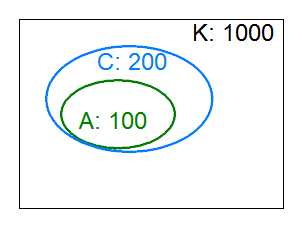
\includegraphics[scale=0.3] {img/table-img2.png}}
&
\begin{tabular}{l l}accuracy& 50\%\\\\ recall & 100\%\end{tabular}
& 90 \% & 66.7 \% & 75 \% & 50 \% \\ \hline 

\raisebox{-.5\height}{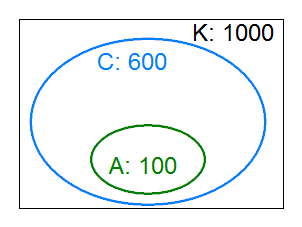
\includegraphics[scale=0.3] {img/table-img3.png}}
& 
\begin{tabular}{l l}accuracy& 16.7\%\\\\ recall & 100\%\end{tabular}
& 50 \% & 28.6 \% & 58.3 \% & 16.7 \% \\ \hline 


\raisebox{-.5\height}{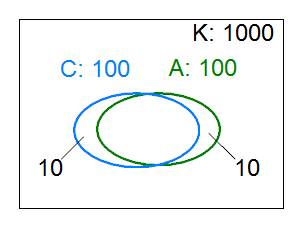
\includegraphics[scale=0.3] {img/table-img4.png}}
& 
\begin{tabular}{l l}accuracy& 90\%\\\\ recall & 90\%\end{tabular}
& 98 \% & 90 \% & 90 \% & 81.8 \% \\ \hline 

\raisebox{-.5\height}{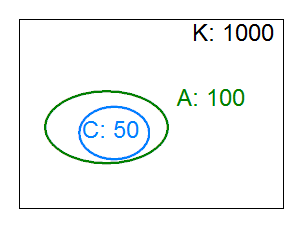
\includegraphics[scale=0.3] {img/table-img5.png}}
& 
\begin{tabular}{l l}accuracy& 50\%\\\\ recall & 100\%\end{tabular}
& 95 \% & 66.7 \% & 75 \% & 50 \% \\ \hline 

\end{tabular}
\end{table*}

\subsubsection*{Subclass and Disjointness of classes}
This query evaluates all individuals (\texttt{?ind}) and checks if they are
instance of the user-defined class definition in \texttt{\$class}. In this
query, a higher value indicates a better candidate for a superclass. 
Lower values indicate possible disjointness.
 
\begin{lstlisting} 
SELECT ?type (COUNT(?ind ) AS ?count ) WHERE {
	?ind a <$class >.
	?ind a ?type .
} GROUP BY ?type
\end{lstlisting}

\subsubsection*{Subsumption and Disjointness of properties}
A somewhat similar query can be used to learn subsumption and disjointness of
\emph{predicates}.

\begin{lstlisting} 
SELECT ?p (COUNT(?s ) AS ?count ) WHERE {
	?s ?p ?o .
	?s <$property> ?o .
} GROUP BY ?p
\end{lstlisting}

\subsubsection*{Domain and Range of properties}
A query for the domain of a property counts the occurrences of subjects of type
\texttt{?type} having the property \texttt{\$property}.

\begin{lstlisting} 
SELECT ?type COUNT(DISTINCT ?ind ) WHERE {
	?ind <$property> ?o .
	?ind a ?type .
} GROUP BY ?type
\end{lstlisting}

The query for the range of \texttt{\$property} works in a similar way. 
For properties you can distinguish between object and data properties.
Here only the queries for object properties are listed.
\begin{lstlisting} 
SELECT ?type (COUNT(DISTINCT ?ind ) AS ?cnt ) WHERE {
	?s <$property> ? ind .
	?ind a ?type .
} GROUP BY ?type
\end{lstlisting}


\subsubsection*{Inverse of Properties}
To check if a property is also inverse, we check the \texttt{\$property} with
subject and object and in swapped position. 
\begin{lstlisting} 
SELECT ?p (COUNT(*) AS ?count ) WHERE {
	?s <$property> ?o .
	?o ?p ?s .
} GROUP BY ?p
\end{lstlisting}


%=====================================================================================
%=====================================================================================
%=====================================================================================
\section{Heuristics}
% Paper 1


\subsection{Finding the right heuristic}
A heuristic measures how well a given class expression fits the learning
problem.\cite{paper1}
To test an algorithm we must have positive and negative examples. As we want to
describe class $A$ with the expression $C$, we can consider every instance of
$A$ as a positive and everything else as negative examples.
The predictive accuracy can be described as:\vspace{9pt}\\
\centerline{
$
predacc(C) = 1 - \frac{|R(A) \setminus R(C)| + |R(C) \setminus R(A)|}{n} \quad n
= |Ind(K)| $
}\vspace{9pt}
Here, Ind(K) stands for the set of individuals in the knowledge base. $R(A)
\setminus R(C)$ are the false negatives whereas $R(C) \setminus R(A)$ are the
false positives. \\
As you can see in Figure 1, for the term \emph{precision} we
consider the intersection of $A$ and $C$ ($R(A) \cap R(C)$) and the false
positive. In other words, how many individuals are rightful considered in our
class expression $C$.\\
For the other term \emph{recall} we consider again the intersection of $A$ and
$C$ and the false negatives. This score tells us how many of the individuals in
$A$ we can describe with our class expression $C$.

Table 1 compares the score of four different heuristics.
They are:
\begin{itemize}
  \item{\textbf{pred. acc.}} The formula for the predictive accuracy was shown
  above.
  \item{\textbf{F-Measure}} The F-Measure is defined as the harmonic mean of
  precision and recall. It can be weighted by a factor $\beta$, the authors in
  \cite{paper1} choose 3 for $\beta$ for learning super classes, which gives
  recall a higher weight than precision.\\
  $F\mymathhyphen Measure = \frac{\beta + 1}{\frac{\beta}{recall} +
  \frac{1}{precision}}$
  \item{\textbf{A-Measure}} For the A-Measure we choose the arithmetic mean of
  precision and recall.\\
  $A\mymathhyphen Measure = \frac{precision + recall }{2}$
  \item{\textbf{Jaccard}} The Jaccard index is well known for comparing two
  sets.
  It is defined as the size of the intersection divided by the size of the union
  of the sets. $Jaccard(A,B) = \frac{|A \cap C|}{|A \cup C|}$
\end{itemize}



%=====================================================================================
%=====================================================================================
%=====================================================================================
\subsection{Efficient heuristic computation}
For big knowledge base the performance and efficiency of the algorithm is
crucial. To compute and test class expression, many retrieval operations are
performed. To minimize the cost and improve the performance, the authors in
\cite{paper1} provide three optimisations:
\begin{itemize}
  \item{\textbf{Reduction of instance checks}} 
  The obvious choice is to reduce the number of instance checks required to test
  expressions. Assuming that we want to learn an equivalence axiom for class A
  with the super class A': Instead of checking every individual of the knowledge
  graph we can restrict our retrieval operation to instances of A'.
  
  \item{\textbf{Approximate and closed world reasoning}} 
  To deal with the very high number of instance checks against the knowledge
  base, CELOE uses a special reasoner.\cite{paper1} It uses an approximate and
  incomplete reasoning for fast instance checks (FIC). The reasoner depends on
  the first run on a standard OWL reasoner to check instances and property
  relationships. The result of this first reasoning is stored in memory for fast
  (but approximated) instance checks. The reasoner follows a closed world
  assumption.
  
  \item{\textbf{Stochastic coverage computation}} 
  This optimisation again reduces the necessary instance checks. Looking at the
  different heuristics, we can see that $|R(A)|$ needs to be computed only once
  whereas e.g. the expensive expression $R(A) \cap R(C)$ is computed for every
  different $C$. To improve performance we can try to approximate the result by
  testing randomly drawn objects and checking if we are sufficiently confident
  that our estimation is within a certain bound.
  
  
\end{itemize}


%=====================================================================================
%=====================================================================================
%=====================================================================================
\section{Evaluation}
To evaluate the methods of class learning, the authors of \cite{paper1} tested
their algorithm on a variety of real world ontologies of different sizes and
domains. The goal of the evaluation consisted of 3 parts: determine the
influence of reasoning and heuristics on suggestions, test the performance and
efficiency on large real world ontologies and to test the accuracy of
approximations described in section 5.2.

To perform the evaluation, the authors in \cite{paper1} wrote a dedicated plugin
for the Prot�g� editor. The plugin first looks for classes with enough
instances. For each of these classes they ran the CELOE algorithm to generate
suggestions for definitions. Here they tested two different reasoner and the
previously described heuristics. The results of these tests were
categorized in three main categories: (1) the suggestion improves the ontology
(improvement), (2) the suggestion does not improve the ontology and therefore
should not be added to the ontology (not acceptable), (3) adding the suggestion
results in a modelling error (error).
A small part of the results is shown in Table 2, the full
evaluation results are shown in \cite{paper1}.
\begin{table}[ht]
\centering
\label{table-eval}
\caption{Evaluation results of \cite{paper1}. Accuracy of different heuristics.}
\begin{tabular}{|p{3.3 cm} p{1 cm} p{1 cm} p{1.3 cm} |} \hline
\textbf{Reasoner/heuristic} & \textbf{Improv.} & \textbf{Not acc.}
& \textbf{missed Improv.} \\\hline

Pellet/F-Measure 		& 16.70 & 64.66 & 14.95 \\
Pellet/A-Measure 		& 16.70 & 64.66 & 14.95 \\
Pellet/pred.acc. 		& 16.59 & 64.93 & 15.22 \\\hline
Pellet FIC/F-Measure 	& 36.60 & 52.62 & 1.90 \\
Pellet FIC/A-Measure 	& 36.19 & 52.84 & 1.63 \\
Pellet FIC/pred.acc. 	& 32.99 & 52.58 & 4.35 \\
\hline
\end{tabular}
\end{table}

The second evaluation results were based on the performance of the approximation
reasoner as described in section 5.2. The tests showed that an approximation
lead to significant performance improvement, this is especially the case for
larger ontologies. The time required to test a class expression showed smaller
variations and a performance gain of several orders of magnitudes has been
achieved. The approximation has shown to be very accurate and had hardly any
influence on the learning algorithm.

Preliminary Evaluation has also been done in \cite{paper2} for OWL axiom
enrichment. The authors choose DBpedia to test their algorithms. Table
3 shows a small subset of the results.
In \cite{paper2} the evaluation is discussed in great detail. For example the
three newly discovered symmetric object properties in the DBpedia ontology were:
\texttt{dbo:neighboringMunicipaly}, \texttt{dbo:sisterCollege} and
\texttt{dbo:currentPartner}.


\begin{table}[ht]
\centering
\label{table-eval-paper2}
\caption{Evaluation results of \cite{paper2} (combined object and data properties)}
\begin{tabular}{| l l p{1.2 cm} l|} \hline
\textbf{axiom type} & \textbf{recall} & \textbf{new axioms}
& \textbf{precision} \\\hline

SubClassOf 			& 180/185 	& 155  & 75 \% \\
EquivalentClasses 	& 0/0 		& 1812 & 50 \% \\
DisjointClasses		& 0/0 		& 2449 & 100 \% \\
PropertyDomain		& 833/942 	& 1298 & 54 \% \\
PropertyRange		& 291/1032 	& 500  & 46 \% \\
SymmetricProperty	& 0/0 		& 3    & 100 \% \\

\hline
\end{tabular}
\end{table}